
% Beamer document class
\documentclass[xcolor=dvipsnames]{beamer}

% packages
\usepackage[utf8]{inputenc}
\usepackage{latexsym}
\usepackage{graphicx}
\usepackage{mathptmx}
\usepackage{amsmath}
\usepackage{amsfonts}
\usepackage{amssymb}
\usepackage{amsbsy}
\usepackage{amsthm}
\usepackage{algorithmic}

% Set VT theme
\usepackage{pgf}
\logo{\pgfputat{\pgfxy(-0.1,0.1)}{\pgfbox[right,base]{
\includegraphics[height=0.5cm]{../templates/VPIlogo.png}}}}
\newcommand{\nologo}{\setbeamertemplate{logo}{}}
\setbeamercolor*{palette tertiary}{bg=Maroon}
\setbeamercolor{frametitle}{fg=Brown,bg=Maroon!20}
\setbeamercolor{section in head/foot}{bg=Maroon}
\setbeamercolor{author in head/foot}{bg=Maroon}
\setbeamercolor{date in head/foot}{fg=Maroon}
\setbeamercolor{section in toc}{fg=Black}
\setbeamercolor{subsection in toc}{fg=Black}
\setbeamercolor{title}{fg=Black}
\setbeamercolor{item}{fg=Black}
\setbeamercolor{block title}{fg=Black,bg=Maroon!20}
\setbeamercolor{caption name}{fg=Black}
\usefonttheme[onlymath]{serif}

% Title Information
\title{\bf A Locally Convergent Search Technique Using a Delaunay Mesh
Surrogate}
\date{International Conference on Continuous Optimization\\
August, 2019}
\author{Tyler Chang$^\star$, Layne Watson, Thomas Lux}
\institute{Virginia Polytechnic Institute and State University}

\begin{document}

% Make title frame with footnote
\begin{frame}
\vfill
\titlepage
\vfill
\usebeamerfont{institute}$^\star$ corresponding author: \url{thchang@vt.edu}
\end{frame}

% Make ToC
\begin{frame}{Table of Contents}
\tableofcontents
\end{frame}

% Begin first section
\section{Introduction and Problem Definition}
\begin{frame}{Motivation}
$$
\min_{x \in B} \text{ } f(x) \quad\text{where }
B \subset \mathbb{R}^d\text{ is simply bounded}
$$
where $f$ is an expensive black-box function, (i.e., a numerical simulation
or real world experiment).\\ \pause

{\bf Typical solution:}\\ \pause
\begin{itemize}
\item Run global optimizer such as DIRECT search algorithm of Jones et al. \\ \pause
\item For problems that are moderately smooth, DIRECT often converges quickly
to the neighborhood of the solution, but painfully slowly to the
exact solution\\ \pause
\item Refine DIRECT solution using a ``local'' optimizer
\end{itemize}
\end{frame}

\begin{frame}{Goal}
Want the local optimizer to use DIRECT's database.
\end{frame}

\begin{frame}{Statement of the Problem}
$$
\min_{x \in B} \text{ } f(x) \quad\text{where }
B \subset \mathbb{R}^d\text{ is simply bounded}
$$
\begin{itemize}
\item $f$ is an expensive black-box function \\
\pause
\item given a finite dataset of $n$ design points $X$ in
$\mathbb{R}^d$ and $n$ corresponding objective values $Y$ in $\mathbb{R}$\\
\pause
\item suspect that some pair $(x,y)$ from the database is
``in the neighborhood'' of the optima\\
\pause
\item also $x^* = \arg\min_{x\in B}$~$f(x)$ is in the convex hull of $X$.
\end{itemize}
\end{frame}

\section{A Mesh Based Approach}
\begin{frame}{The Mesh Refinement Scheme}
\begin{itemize}
\item In iteration $k$, compute $DT(X^{(k-1)})$, where $X^{(k-1)}$ is the
previous data set (let $X^{(0)} = X$) and $DT(X^{(k-1)})$ is a mesh\\
\pause
\item Judge the ``fitness'' of each element in the mesh
$DT(X^{(k)})$ by the estimated objective value at its center\\
\pause
\item Refine the mesh by evaluating $x^{(k)}$ at the center of element
with the lowest estimated objective value\\
\pause
\item $X^{(k)} = X^{(k-1)} \cup \{x^{(k)}\}$
\end{itemize}
\end{frame}

\begin{frame}{What is the Delaunay Triangulation}
\begin{itemize}
\item Let $P$ be a set of $n$ points in $\mathbb{R}^d$
\item Let $CH(P)$ denote the convex hull of $P$
\item $DT(P)$ (the Delaunay triangulation of $P$) is an 
{\it unstructured simplicial mesh} over $CH(P)$, whose vertex set is $P$
\item The {\it Delaunay triangulation} is a special triangulation, often
considered optimal for interpolation and meshing purposes
\end{itemize}
\begin{center}
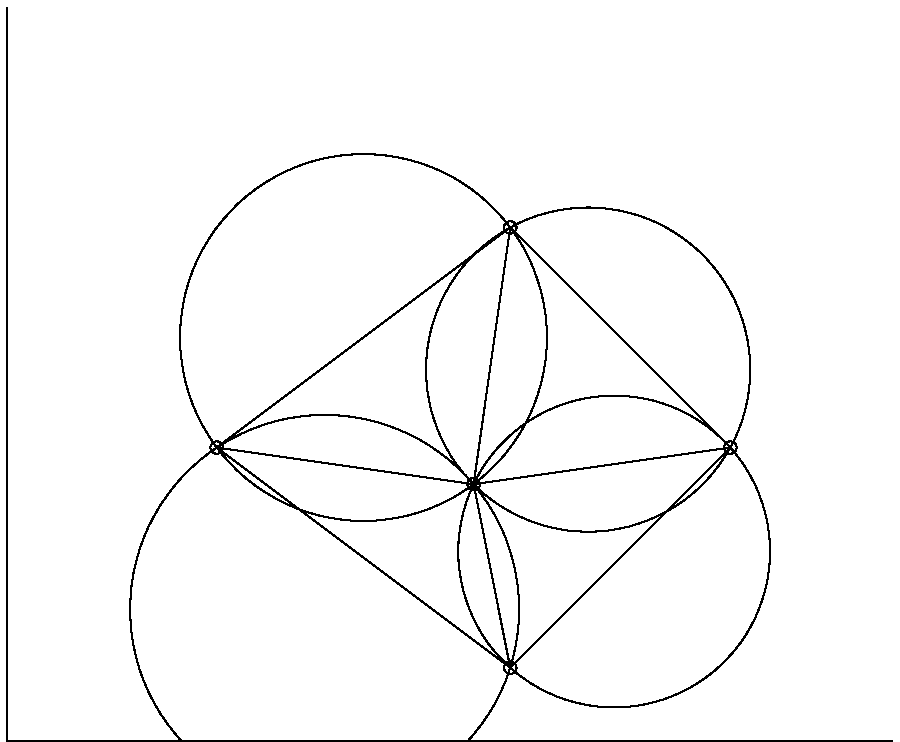
\includegraphics[width=0.4\columnwidth]{../img/delaunay_old/delaunayplane-eps-converted-to.pdf}
\end{center}
\end{frame}
\begin{frame}{Uses}
\begin{itemize}
\item Mesh generation (e.g., for finite element methods or computer graphics)
\item Piecewise linear multivariate interpolation (e.g., for GIS)
\item Topological data analysis
\item Graph theory
\end{itemize}
\begin{center}
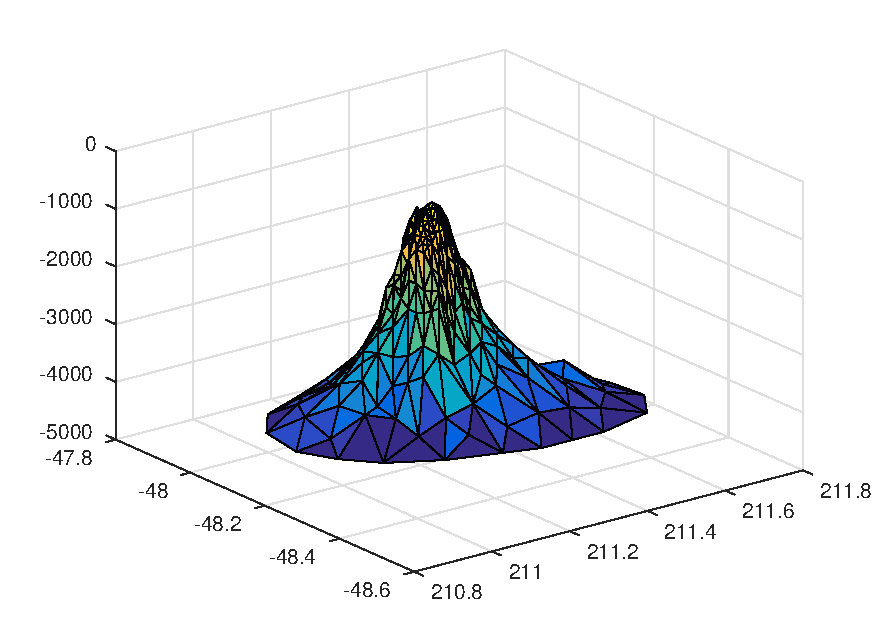
\includegraphics[width=0.4\columnwidth]{../img/delaunay_old/seamount-eps-converted-to.pdf}
\end{center}
\end{frame}

\section{The Surrogate}
\begin{frame}{Linear Interpolation}
\begin{itemize}
\item Let $S$ be a simplex in $DT(P)$ with vertices $\{s_1,\ldots,s_{d+1}\}$
\item Then $\{s_1,\ldots,s_{d+1}\}$ define a plane $\ell$, along which we
can linearly interpolate any $q\in S$
\item Let $w_1,\ldots,w_{d+1}$ be {\it convex weights} such that
$\sum_{i=1}^{d+1} s_i w_i = q$. Then
$$
\hat{f}_S (q) = f(s_1) w_1 + f(s_2) w_2 + \text{ $\ldots$ } + f(s_{d+1})w_{d+1}
$$
\pause
\item $\hat{f}_S$ could also be used to extrapolate for $z \not\in S$, akin
to following the gradient estimate in $S$
\end{itemize}
\end{frame}
\begin{frame}{Gradient Estimates}
Owing to Lux et al.\ (citation pending), the following Lemma:\\
\medskip
Let $f$ be a function whose gradient is $\lambda$ Lipschitz continuous in
the $2$-norm.\\
\smallskip
Let ${\hat g}_S$ be the (constant) gradient field in $S$ with respect to
${\hat f}_S$\\
\smallskip
Then for any vertex $s_j$ of $S$
$$
\|\nabla f(s_j) - {\hat g}_S\|_2 \leq \sqrt{d}\frac{\lambda k^2}{\sigma_d}
$$
where $k$ is the maximum edge length of $S$ and $\sigma_d$ is the smallest
singular value of 
$T = \left[ s_2-s_1\quad \ldots\quad s_{d+1}-s_1 \right]$.\\
\smallskip
{\bf Takeaway:} as the diameter of an element shrinks, its constant gradient
estimate converges to the true gradient
\end{frame}

\begin{frame}{Method for Refinement}
\begin{itemize}
\item For an element in the mesh, the objective value at its center is
voted on using the gradient estimates of its $d+1$ neighbors
(in this work, via averaging)
\item The next function evaluation $x^{(k)}$ is chosen as the center with
the most promising estimate
\end{itemize}
\end{frame}
\begin{frame}{Convergence}
\begin{itemize}
\item Within a neighborhood of the global minima, we would expect to see
many design points sampled (requires proof)
\item Then the estimated gradients converge, and the algorithm converges
similarly to gradient descent
\end{itemize}
\end{frame}

\section{Results}
\begin{frame}{Experiments}
The following preliminary experiments were run for 100 iterations over
objective functions of two design variables using the Delaunay Search
algorithm.\\
\medskip
In all cases, the initial database was taken from a latin hypercube design
of 20 points.\\
\medskip
All functions were shifted so that their global minima has objective
value $f(x^*) = 0$\\
\end{frame}
\begin{frame}{Quadratic}
\begin{center}
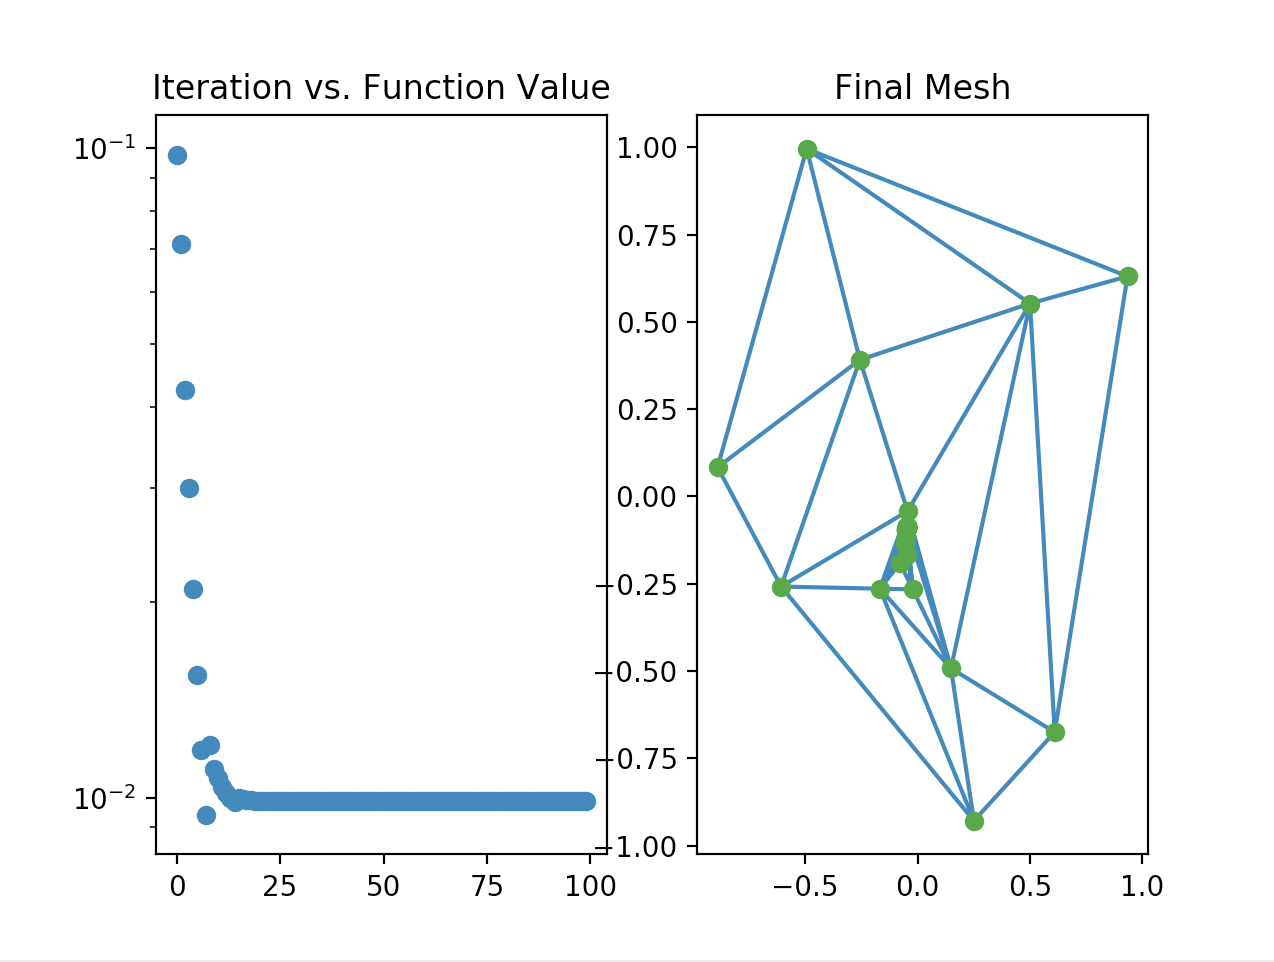
\includegraphics[width=0.8\columnwidth]{../img/delaunay_search/ds-QuadraticError.png}
\end{center}
\end{frame}
\begin{frame}{Rosenbrock}
\begin{center}
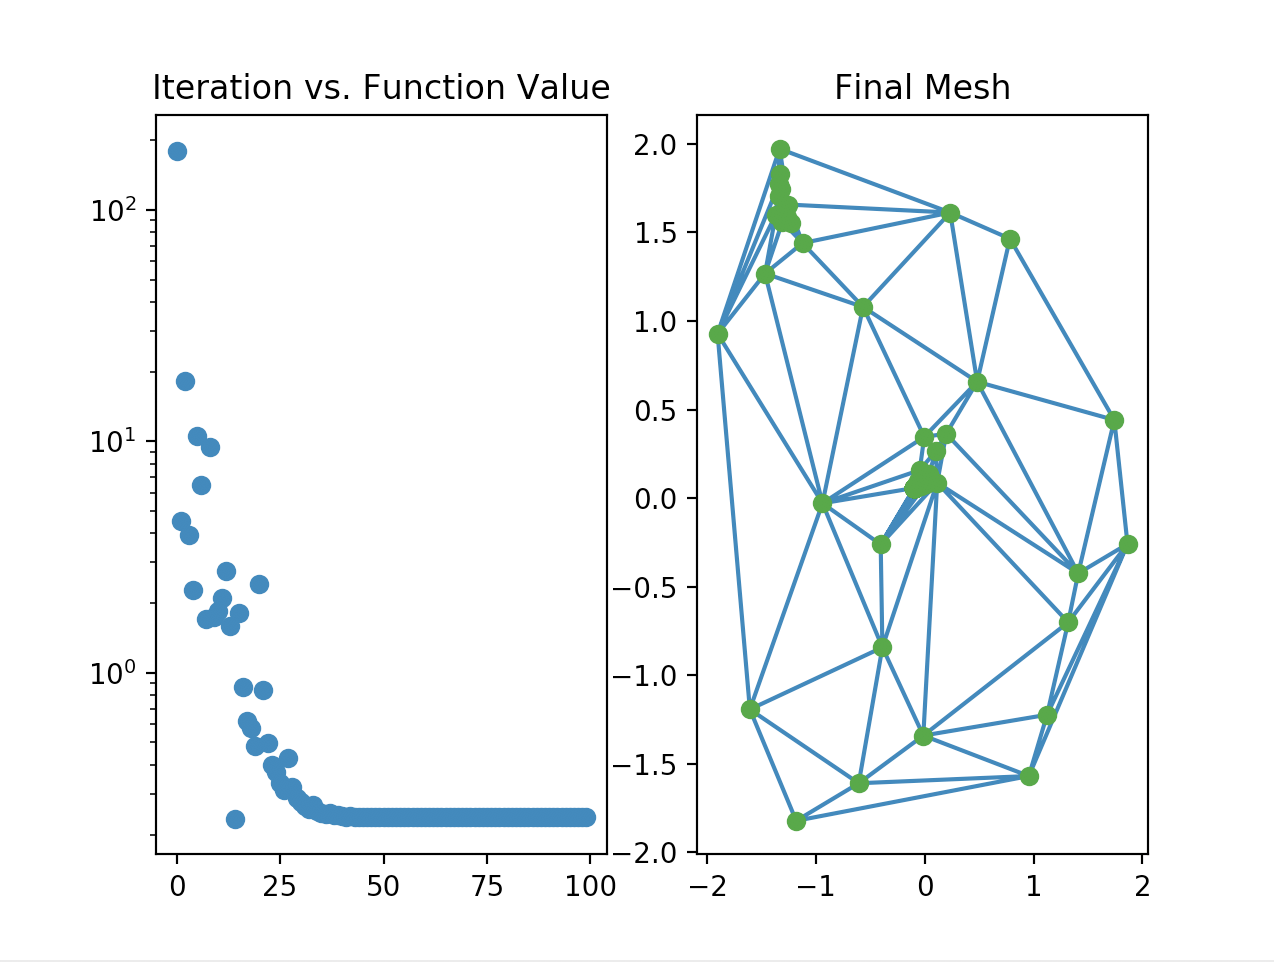
\includegraphics[width=0.8\columnwidth]{../img/delaunay_search/ds-RosenbrockError.png}
\end{center}
\end{frame}
\begin{frame}{Michaelwicz}
\begin{center}
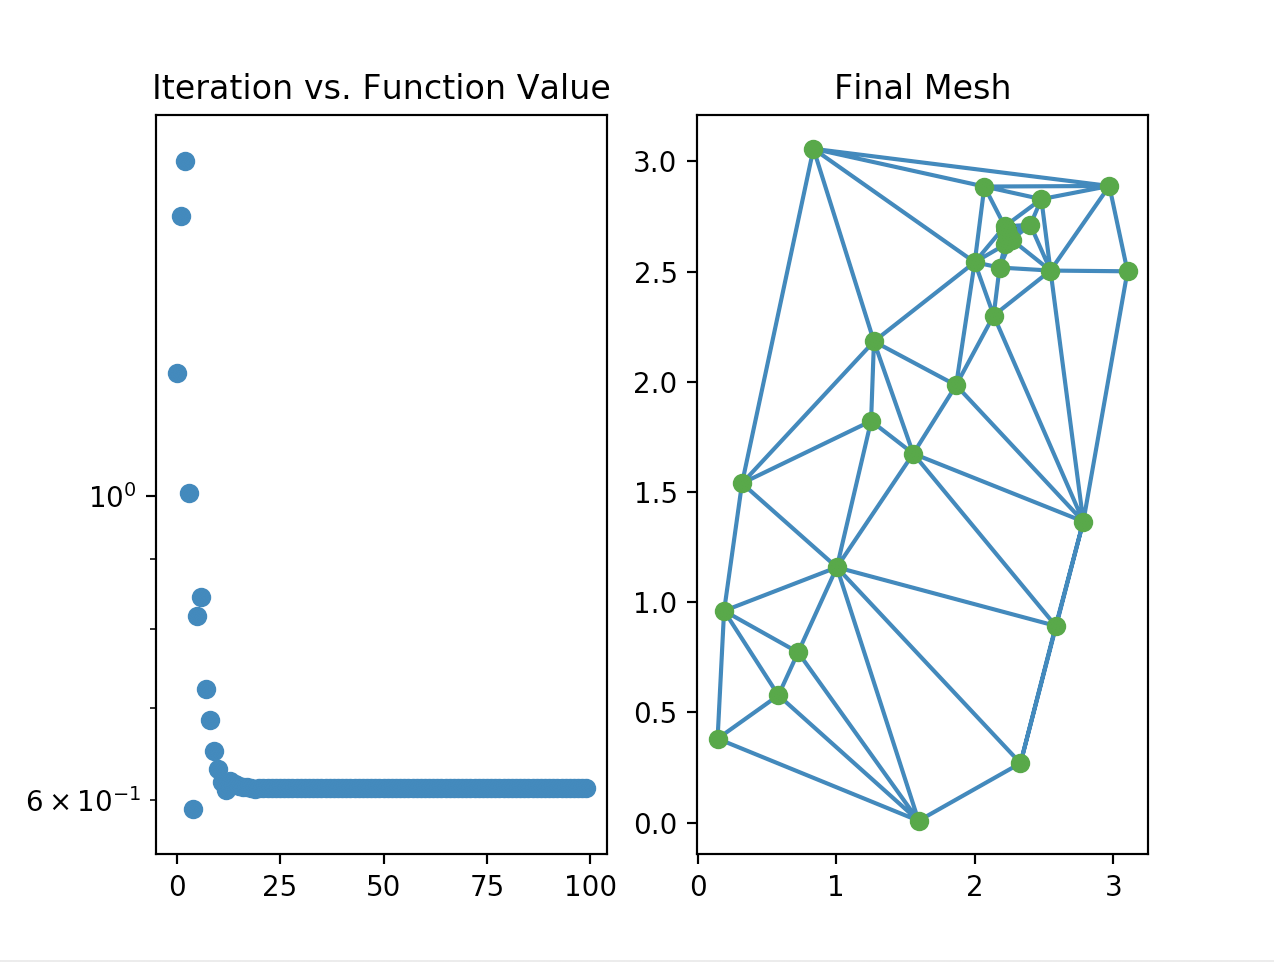
\includegraphics[width=0.8\columnwidth]{../img/delaunay_search/ds-MichaelwiczError.png}
\end{center}
\end{frame}
\begin{frame}{Griewank}
\begin{center}
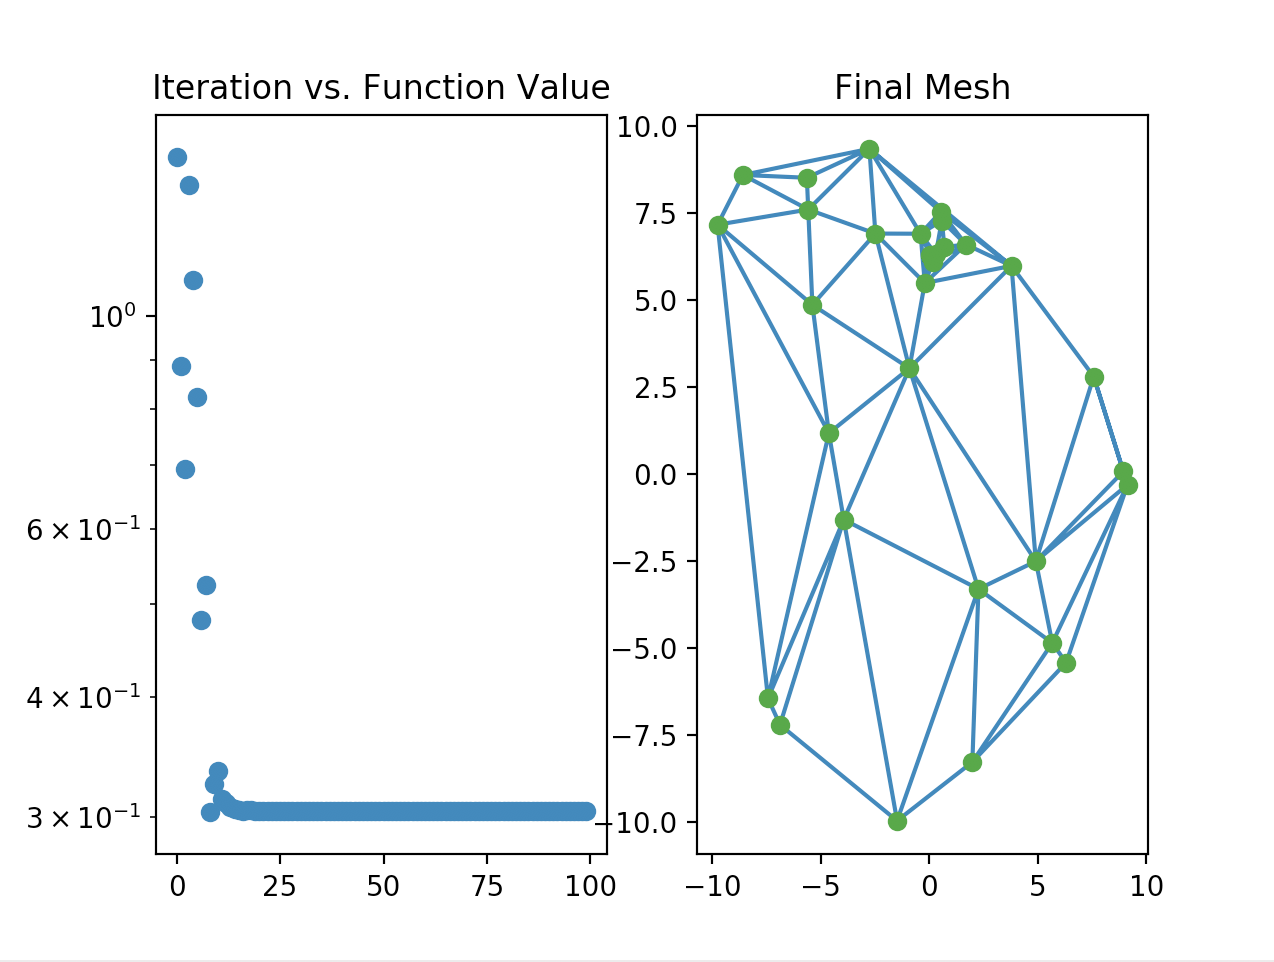
\includegraphics[width=0.8\columnwidth]{../img/delaunay_search/ds-GriewankError.png}
\end{center}
\end{frame}

\section{Future Work}
\begin{frame}{Limitations and Future Works}
\begin{itemize}
\item Prove something about how data will be sampled in the neighborhood of
the current observed minima (to show that the gradient estimates will converge
in a neighborhood of a local minima)
\item Currently, cannot sample outside the convex hull of the initial dataset
$X$. Extensions for when $x^* \not\in CH(X)$. Maybe LP?
\item For $d$ large, computing the entire Delaunay mesh is intractible.
But using some properties of the Delaunay mesh and optimization problem,
we should be able to eliminate many regions from consideration, making this
tractible for relatively large $d$
\end{itemize}
\end{frame}
\begin{frame}
\centering{{\Huge{QUESTIONS?}}}
\end{frame}

\end{document}
              
